\documentclass{beamer}
\usepackage[french]{babel}

\usepackage[utf8]{inputenc} 
\usepackage[T1]{fontenc}
\usepackage{lmodern}
\usepackage{graphicx}
\usepackage{float}
\usepackage{hyperref}
\usepackage{listings}
\usepackage{caption}

\setbeamercovered{transparent}

\newcommand{\bsf}{Baguette\# }
\newcommand{\bs}{B\# }

\title{Approche pratique de la théorie des langages formels. \\ Oral de TIPE}
\author{Charlotte THOMAS}

\begin{document}
    \frame{\titlepage}
    \section{Généralités}
    \begin{frame}
        \frametitle{Résumé}
        Les erreurs de compilation peuvent coûter cher, et parfois se compter en vies humaines, il est donc 
        nécessaire de développer des outils et des théories dans le domaine de la théorie des langages formels 
        pour prévenir les bugs en amont, et protéger des vies et la société.\pause


        Pour illustrer ceci cette présentation se concentre sur le \textit{\bsf} (à prononcer "Baguette Sharp") un langage 
        de programmation exotique avec une syntaxe proche d'un BASIC, basé sur des pâtisseries.
        Le REPL est disponible sur OPAM \textit{opam install baguette-sharp}, le code source est sur \href{https://github.com/coco33920/ocaml-baguettesharp-interpreter}{GitHub}
        sous licence MIT, enfin le site web est disponible à cette adresse \url{https://www.baguettesharp.fr}
    \end{frame}
    
    \begin{frame}
        \frametitle{Tableau des matières}
        \begin{enumerate}
            \item Présentation du langage
            \begin{enumerate}
                \item Présentation Générale
                \item Lexer
                \begin{itemize}
                    \item Lexer
                    \item Lexer - Algorithme 
                \end{itemize}
                \item Parser
                \begin{itemize}
                    \item Parser/AST 
                    \item Parser - Algorithme 
                    \item Parser - Parenthèse ouvrante
                    \item Parser version complète
                \end{itemize}
            \end{enumerate}
            \item Machine de Turing Universelle Binaire 
            \begin{enumerate}
                \item Définition 
                \item Implémentation
                \item Implémentation en \bs
                \item Exemples et résultats
                \begin{itemize}
                    \item Bit-Shift
                    \item Binary Adder
                    \item Overflow
                \end{itemize}
            \end{enumerate}
        \end{enumerate}
    \end{frame}

    \begin{frame}
        \frametitle{Présentation générale}
        
        Le \bsf a une syntaxe proche d'un BASIC à quelques exceptions près, qui ont été choisies dès le début.
        \begin{itemize}
            \item<1> L'absence d'opérateurs INFIX (par exemple 1+2)
            \item<2> Toutes les instructions ont un nom de pâtisserie (pour le rendre moins simple et plus éxotique)
            \item<3> Chaque structure (condition, boucle, fonction) a une syntaxe complètement différente que les autres
            \item<4> Enfin, tous les algorithmes ainsi que leurs implémentations ont été codées à la main sans avoir recours aux bibliothèques 
            en OCaml (telles que OCamlLex et Menhir).
        \end{itemize}
    \end{frame}

    \begin{frame}
        \frametitle{Algorithmes}
        Le \bs est pour l'instant uniquement interprété il passe donc par plusieurs étapes standard afin d'être évalué correctement
        \begin{itemize}
            \item<1> Le fichier source / la ligne de code est lue est passée par
            le \textbf{lexer} pour en former une liste de token
            \item<2> La liste de Token est passée par le \textbf{parser} pour former un arbre de syntaxe abstraite (AST)
            \item<3> L'AST est ensuite interprété en suivant la structure de l'arbre en profondeur (un algorithme sensiblement proche d'un DFS)
        \end{itemize}
    \end{frame}

    \begin{frame}
        \frametitle{Lexer}
        La liste complète des tokens est disponible dans base/token.ml,
        \begin{figure}[H]
            \center
            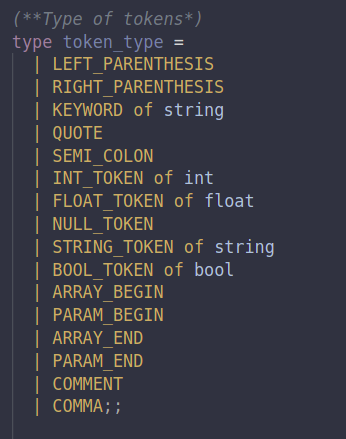
\includegraphics[width=0.5\textwidth]{img/tokentype.png}
            \caption{Type des tokens}
        \end{figure}
    \end{frame}

    \begin{frame}
        \frametitle{Lexer - Algorithme}
        \begin{enumerate}
            \item<1> Le fichier d'entrée est lu et les sauts de ligne sont enlevés
            \item<2> La chaîne de caractère est coupée en une liste de mot (à chaque blanc)
            \item<3> Chaque mot est injecté à un algorithme de reconnaissance des \textit{tokens}
            \item<4> On construit récursivement comme ceci la liste des tokens
            \item<5> On renvoie la liste renversée (pour conserver l'ordre de lecture)
        \end{enumerate}
        \begin{figure}[H]
            \center
            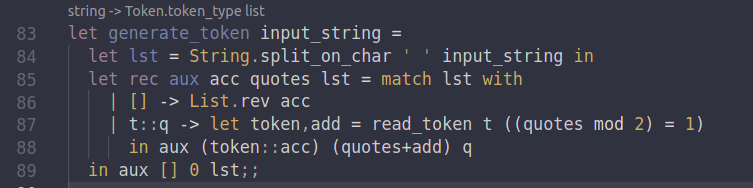
\includegraphics[width=0.7\textwidth]{img/implem.png}
            \caption{Implémentation du \textit{lexer} principal}
        \end{figure}
    \end{frame}

    \begin{frame}
        \frametitle{Parser/AST}

        L'AST en lui-même est un arbre à n-enfant défini comme ceci en OCaml, bien que générique dans la définition, 
        le type utilisé en pratique est un \textit{parameters ast} 
        \begin{figure}[H]
            \center
            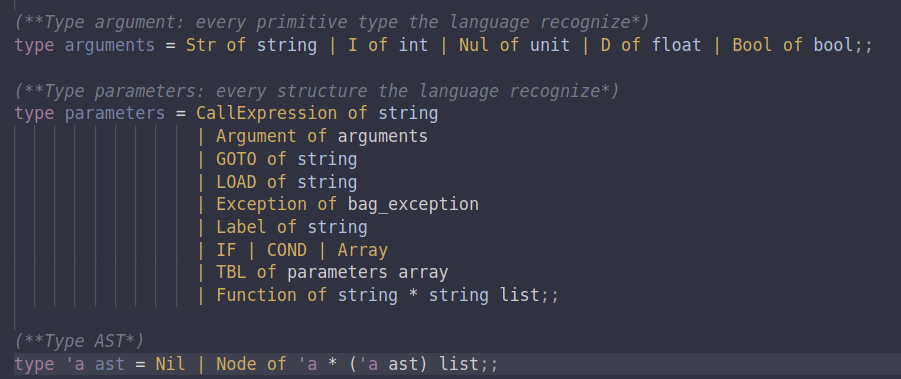
\includegraphics[width=0.7\textwidth]{img/type.png}
            \caption{Type de l'AST et des paramètres}
        \end{figure}
    \end{frame}

    \begin{frame}
        \frametitle{Parser - Algorithme}
        L'algorithme du \textit{parser} est assez classique, bien qu'il ne soit pas exactement un algorithme connu (pour tout faire depuis
        zéro sans utiliser d'algorithme connu/classiques) il est classique pour un parser récursif en mémorisant le \textit{dernier token} lu
        pour pouvoir calculer le contexte, ci-après l'implémentation du parsing des parenthèses ouvrantes, qui va être présenté en détail
        \begin{figure}[H]
            \center
            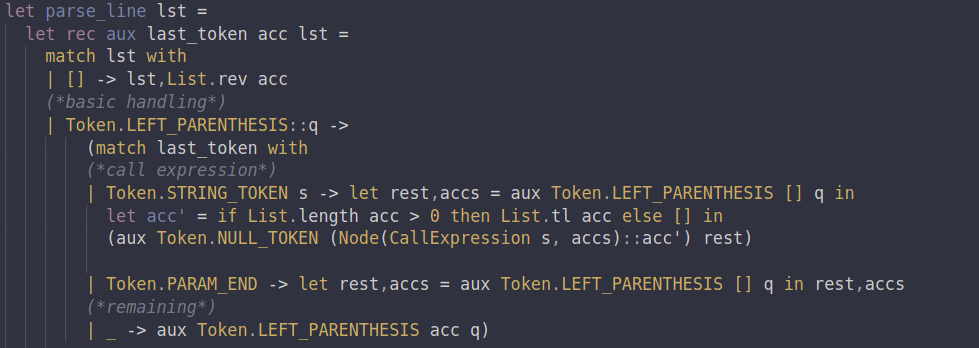
\includegraphics[width=0.7\textwidth]{img/parenth.png}
            \caption{Handler de la lecture du token de parenthèse ouvrante}
        \end{figure}
    \end{frame}

    \begin{frame}
        \frametitle{Parser - Parenthèse ouvrante}
        La condition de sortie est généralement une parenthèse fermante, en effet la validation du parenthésage est automatique lors de l'interprétation,
        il est donc présumé que le programme est bien parenthésé.
        \begin{enumerate}
            \item<1> On lit une parenthèse ouvrante, on match le token précédent
            \item<2> Si c'est une chaîne de caractère on décide que c'est une instruction, une \textit{call expression}
            \begin{itemize}
                \item<3> On relance l'algorithme de parsing avec un accumulateur vide (pour avoir les paramètres de l'expression)
                \item<4> On supprime la tête de la liste (qui est généralement le nom de l'instruction) si la liste est non-vide 
                \item<5> On continue l'algorithme sur la suite de la liste de token en ajoutant une Node \textit{call expression} à l'arbre accumulé
            \end{itemize}
            \item<6> Si le dernier token est une accolade fermante (qui signifie la fin des paramètres d'une déclaration de fonction) alors on 
            relance l'algorithme et on renvoie l'accumulateur et le reste de la liste de token
            \item<7> Sinon on continue l'algorithme en sautant la parenthèse
        \end{enumerate} 
    \end{frame}

    \begin{frame}[allowframebreaks]
        \frametitle{Parser version complète}
        (À sauter sauf si demande du jury).

        En réalité l'algorithme est bien plus gros, la parenthèse ouvrante n'est qu'un moment clef parmi d'autre, l'algorithme entier est expliqué ci-dessous si besoin.
        \begin{enumerate}
            \item On vérifie les conditions de sortie (liste vide)
            \item Si on lit une parenthèse ouvrante
            \begin{enumerate}
                \item On match le token précédent
                \item Si c'est une chaîne de caractère on décide que c'est une instruction, une \textit{call expression}
                \begin{itemize}
                    \item On relance l'algorithme de parsing avec un accumulateur vide (pour avoir les paramètres de l'expression)
                    \item On supprime la tête de la liste (qui est généralement le nom de l'instruction) si la liste est non-vide 
                    \item On continue l'algorithme sur la suite de la liste de token en ajoutant une Node \textit{call expression} à l'arbre accumulé
                \end{itemize}
                \item Si le dernier token est une accolade fermante (qui signifie la fin des paramètres d'une déclaration de fonction) alors on 
                relance l'algorithme et on renvoie l'accumulateur et le reste de la liste de token
                \item Sinon on continue l'algorithme en sautant la parenthèse
            \end{enumerate}
            \item Si on lit une accolade ouvrante (paramètre de fonction)
            \begin{enumerate}
                \item On match le token précédent
                \item Si c'est une chaîne de caractère
                \begin{itemize}
                    \item On relance l'algorithme de parsing avec un accumulateur vide (pour avoir les paramètres de l'expression)
                    \item On supprime la tête de la liste (qui est généralement le nom de l'instruction) si la liste est non-vide 
                    \item On continue l'algorithme sur la suite de la liste de token en ajoutant une Node \textit{call expression} à l'arbre accumulé 
                \end{itemize}
                \item Sinon on continue en sautant l'accolade
            \end{enumerate}
            \item Si on est sur une accolade fermante on sort avec l'accumulateur et la liste restante
            \item Si on est sur un début de tableau (crochet ouvrant) alors on appelle le parser en profondeur et on continue 
            en ajoutant une Node de type Array à l'accumulateur
            \item Si on tombe sur une parenthèse fermante on sort avec l'accumulateur et la liste restante
            \item Si on tombe sur une fin de tableau (crochet fermant) idem
            \item Si on tombe sur un point virgule, idem
            \item Si on tombe sur une virgule, on la saute (pour prendre en compte le lexer secondaire)
            \item Si on tombe sur un IF alors on appelle le parser en profondeur et on ajoute une Node IF à l'accumulateur
            \item Si on tombe sur un BEGIN on vérifie que le token précédent est un keyword et on continue
            \item Si on tombe sur un THEN on vérifie qu'on a un IF avant et si oui on ajoute une node de type condition
            \item Si on tombe sur un LABEL alors on part en profondeur pour le nom du label et son contenu et on ajoute une node de type label
            \item Si on tombe sur un GOTO alors on vérifie le nom et on ajoute une node de type GOTO
            \item Idem pour un LOAD
            \item Si on tombe sur un QUOTE alors on construit la chaîne de caractère jusqu'à tomber sur le quote fermant
            \item Si on tombe sur un string, idem
            \item Si on tombe sur un int, on ajoute une node de type argument de type int
            \item Si on tombe sur un float, on ajoute une node de type argument de type float
            \item Si on tombe sur un boolean, on ajoute une node de type argument de type boolean
            \item Sinon on sort en renvoyant la liste et l'accumulateur
        \end{enumerate}
    \end{frame}

    \begin{frame}[allowframebreaks]
        \frametitle{Machine de Turing Universelle Binaire - Définition}
        Bien entendu créer un langage s'avère uniquement utile si on est capable d'écrire une quantité intéressante d'algorithme dans 
        ce langage, pour cela l'outil théorique de la \textit{Machine de Turing Universelle} est très utile.\newline

        \pause
        
        Une machine de Turing est un \textit{modèle abstrait}, pensé originellement par le précurseur des sciences de l'informatique 
        et mathématicien \textbf{Alan Turing} lors de ses recherches sur la \textit{calculabilité}, une définition intuitive d'une telle machine 
        est par une tête de lecture et un ruban de longueur infini à droite, la tête de lecture lit la "case" et d'après un tableau d'action bouge à droite/gauche/pas, écris 
        quelque chose sur la case (ou pas) et change la machine d'état.\newline 
    \end{frame}

    \begin{frame}
        \frametitle{Machine de Turing Universelle Binaire - Définition}
        Une définition formelle est énoncé par Lewis dans \textit{Elements of the Theory of Computation} en 1982, il définit une machine de Turing 
        comme un 5-uplet $(K,\Sigma,\delta,s,H)$ avec $K$ l'ensemble fini d'états possible de la machine, $\Sigma$ est l'alphabet qui contient 
        le caractère nul et le caractère marquant le début du ruban, $s \in K$ est l'état initial de la machine, $\delta$ est la fonction 
        de transition des états formellement $(K - H) \times \Sigma \to K \times (\Sigma \cup \{\leftarrow,\rightarrow\})$
        (elle prend en entrée un couple formé d'un état non sortant et d'un état du ruban lu et 
        renvoi un couple du nouvel état de la machine et du nouvel état à écrire ou s'il faut bouger à gauche ou à droite, ce qui 
        revient à un nouvel état à écrire ET s'il faut bouger à gauche/droite), et enfin $H \subset K$ est l'ensemble des états 
        finaux dit "de halte". (\textit{Elements of the Theory of Computation, Chapter 4, Definition 4.1.1, p. 181})\newline
    \end{frame}

    \begin{frame}[allowframebreaks]
        \frametitle{Machine de Turing Universelle Binaire - Implémentation}
        Ici est utilisé une machine de Turing dites, \textit{binaire}, avec le caractère $2$ comme caractère vide, 
        il y a un seul état sortant dénoté $\bar{H}$ (pour éviter de le confondre avec le H de la définition, ils sont ensuite confondu) 
        les autres états sont des entiers. 
        Les caractères $r,l,*$ respectivement signifient aller à droite, aller à gauche, et ne pas bouger.
        Enfin la fonction $\delta$ est découpé en trois fonctions $\delta_1,\delta_2,\delta_3$ donnant respectivement 
        le nouvel état, ce qu'il faut écrire sur le ruban, et comment il faut bouger la tête
         on a donc quelque chose comme ci-dessous. 
         On utilise des matrices pour les fonctions (matrice de tailles (n,3)), un nombre pour l'étape actuelle et une chaîne de caractère pour le ruban,
         tout ceci pour pouvoir être implémenté en \bsf!
        \begin{align*}
            K &= H \cup Q && Q \subset \mathbb{N} \\
            \Sigma &= \{0,1,2\} \\ 
            s &= 0 \\ 
            H &= \{\bar{H}\} \\ 
            \delta_1 &: Q \times \Sigma \to K \\ 
            \delta_2 &: Q \times \Sigma \to \Sigma \\ 
            \delta_3 &: Q \times \Sigma \to \{r,l,*\}
        \end{align*}
    \end{frame}

    \begin{frame}[allowframebreaks]
        \frametitle{Machine de Turing Universelle Binaire - Implémentation en \bs }
        En omettant la boucle lisant l'entrée clavier pour le programme l'important est la partie \textit{étape} dont le code en \bs est 
        disponible sur le compte Github dans le fichier \textit{examples/turing.baguette} à la ligne $26$
        La boucle principale de \textit{runtime} s'éxécute juste après la lecture du programme qui a lieu après l'initialisation, et ce, tant que l'état de la machine n'est pas $H$
        \begin{figure}[H]
            \center 
            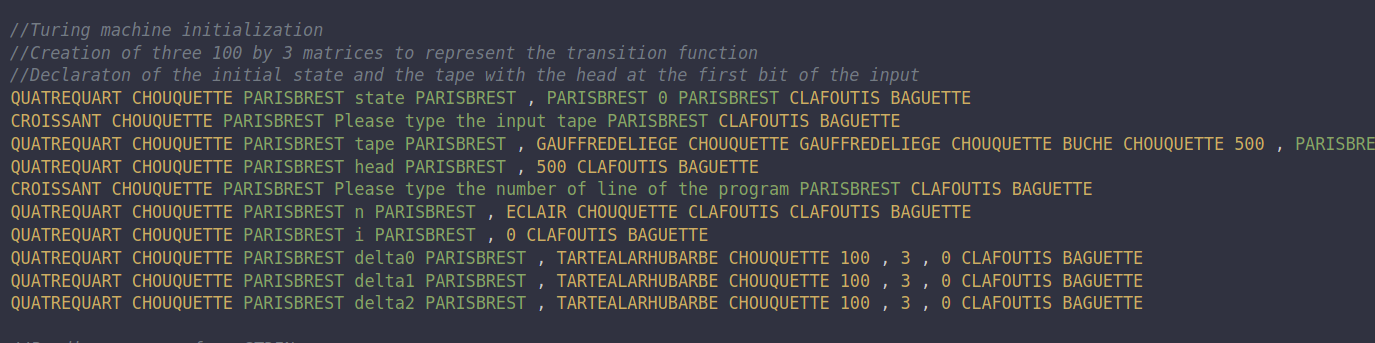
\includegraphics[width=0.7\textwidth]{img/init.png}
            \caption{Initialisation de la machine}
        \end{figure}
        \begin{figure}[H]
            \center
            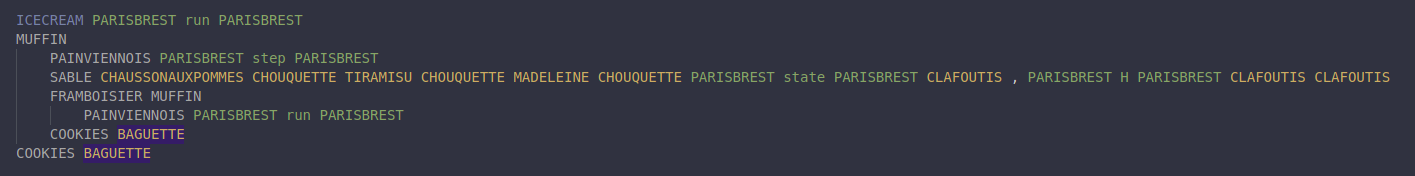
\includegraphics[width=0.7\textwidth]{img/runtime.png}
            \caption{Runtime}
        \end{figure}
    \end{frame}

    \begin{frame}
        \frametitle{Résultats - Bitshift}
        Maintenant on peut présenter quelques programmes qui tourne sur cette machine de Turing. Sous la forme d'algorithme et l'automate 
        d'état associé. Ici un bitshift,
        \begin{itemize}
            \item<1> Si on est dans l'état 0 et qu'on lit un 0 on écrit un 0, on bouge à droite, et on reste dans l'état 0
            \item<2> Si on est dans l'état 1 et qu'on lit un 1 on écrit un 1, on bouge à droite, et on reste dans l'état 0
            \item<3> Si on est dans l'état 0 et qu'on lit un 2 on écrit un 0, on ne bouge pas et passe en état "H"
        \end{itemize}
        \begin{figure}[H]
            \center
            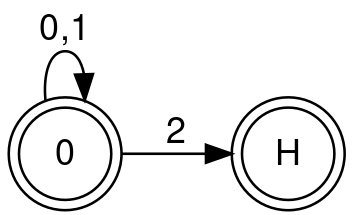
\includegraphics[width=0.5\textwidth]{img/automata1.png}
            \caption{Automate d'état du bitshift}
        \end{figure}
    \end{frame}
    \begin{frame}
        \frametitle{Résultats - Adder}
        Ou encore un binary adder qui en automate d'état rend 
        \begin{figure}
            \center 
            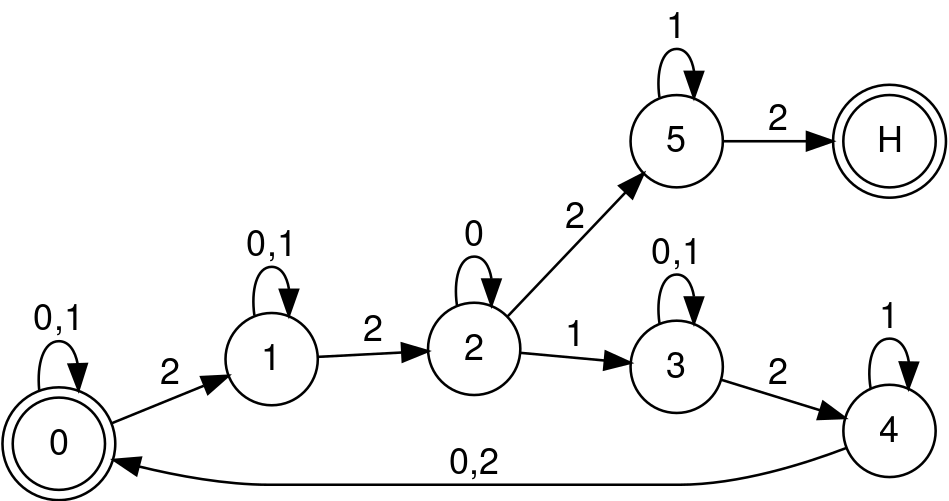
\includegraphics[width=0.7\textwidth]{img/automata2.png}
            \caption{Automate d'état du binary adder}
        \end{figure}
    \end{frame}
\end{document}
